\chapter{Homographien}
\label{sec:homographien} 

Im vorherigen Kapitel wurde mathematisch die Projektion eines 3D-Punktes in einen 2D-Bildpunkt auf einem Kamerasensor durch Koordinatentransformation aufgezeigt. Im nächsten Schritt soll die Beziehung zwischen dem projizierten 3D-Punkt in zwei perspektivische Kameras und den entstehenden 2D-Bildpunkten genauer erläutert werden. Die 2D-Bilder des projizierten 3D-Punktes sind abhängig vom Aufbau der abgebildeten Szene und den Positionen und Ausrichtungen der Kameras\cite{Elements}. Die Beziehung zwischen einem 3D-Punkt und seinen projektionen auf zwei Kameras, kann in einer sogenannten Homographie beschrieben werden. Die Homographie gilt jedoch nur für die Projektion einer planaren Szene im 3D-Raum auf auf zwei Kamerasensoren. Als Homographie wird eine projektive Transformation zwischen zwei Ebenen bezeichnet. Dabei bleiben Kollinearitäten und die Reihenfolge von Punkten auf Geraden, wie zum Beispiel Schnittpunkte mit anderen Geraden, erhalten. Bei den Ebenen handelt sich in diesem Fall um die Bildebenen des Kameramodells. Aufgrund dieser Ebenenannahme, kann solch eine projektive Transformation durch eine 3x3-Homograohiematrix ausgedrückt werden\cite{Roser}. Die Homograohiematrix $H$, projiziert jede Figur in eine Figur gleicher projektiver Entsprechung\cite{HZ,Elements}. Sind die Punkte $A',B',C'$ und $D'$ die projektiven Bilder eines Systems von vier kollinearen Punkten, so ist $(A',B',C',D') = (A,B,C,D)$\cite{Peiffer}. Der Grund warum Homographien in dieser Arbeti eingeführt werden ist, dass sie elementar sind wenn es darum geht Transformationen auf den Bildebenen der Kamera durchzuführen, wie es im Kapitel \nameref{sec:rectification} für die geometrische Entzerrung zweier Bilder von Nöten ist.Außerde bildet ihre geometrische Herleitung eine gute Brücke zur \nameref{sec:epipolar}, welche im nachfolgenden Kapitel vorgestellt wird und der Elementare Baustein für die Stereobildanalyse bildet. Mit Hilfe der Homography ist es möglich eine Beziehung zwischen den zwei projizierten 2D-Bildpunkten herzuleiten, ohne das intrinsische Parameter in Form einer Kamermatrix $K$ noch die extrisischen Parameter in Form der Matrix $R$ bekannt sind\cite{HZ,Elements}.  Diese können dann wiederum aus der, durch die Bildpunkte beider Kameras, entstandenen Homographiematrix geschätzt werden\cite{HZ}. Die Homographie fasst die Transformationen wie Rotation und Translation, sowie die jeweiligen Abbildungsmatrizen der Kameras in einer 3x3-Matrix zusammen.\cite{Elements,Peiffer}. 


Es seien \ensuremath{m_{\tau} = \begin{pmatrix}
		m_{\tau,1}\\m_{\tau,2}\\m_{\tau,3}
\end{pmatrix}} die homogenen Koordinaten eines Punktes auf der Bildebene$(I,\tau)$ und \ensuremath{m'_{\tau'} = \begin{pmatrix}
m'_{\tau',1}\\m'_{\tau',2}\\m'_{\tau',3}
\end{pmatrix}} ein Punkt der projektiv transformierten Bildebene $(I',\tau')$. Dann gilt

\begin{gather}
	m'_{\tau'} = Hm_{\tau}\\
	Hm_{\tau} = \begin{bmatrix}
	{h_1}^T \cdot m_{\tau}\\{h_2}^T \cdot m_{\tau}\\{h_3}^T \cdot m_{\tau}
	\end{bmatrix} \\
	\leadsto 
	m'_{\tau'}= Hm_{\tau}= \begin{bmatrix}
	h_{11}m_{\tau,1}+h_{12}m_{\tau,2}+h_{13}m_{\tau,3}\\
	h_{21}m_{\tau,1}+h_{22}m_{\tau,2}+h_{23}m_{\tau,3}\\
	h_{31}m_{\tau,1}+h_{32}m_{\tau,2}+h_{33}m_{\tau,3}
	\end{bmatrix}\\
	\leadsto 
	H=\begin{bmatrix}
	h_{11}&h_{12}&h_{13}\\
	h_{21}&h_{22}&h_{23}\\
	h_{31}&h_{32}&h_{33}
	\end{bmatrix}
\end{gather}

Dabei müssen die Koeffizienten so geartet sein, dass die zugehörige Transformation umkehrbar ist\cite{HZ}\cite{Peiffer}.
\begin{gather}
	m'_{\tau'}=Hm_\tau\\
	m_\tau= H^{-1}m'_{\tau}
\end{gather}\\


(GRAFIK NOCH ANPASSEN MIT $m_\beta$ etc)\\


\begin{figure}[!htb]
	\minipage{0.48\textwidth}
	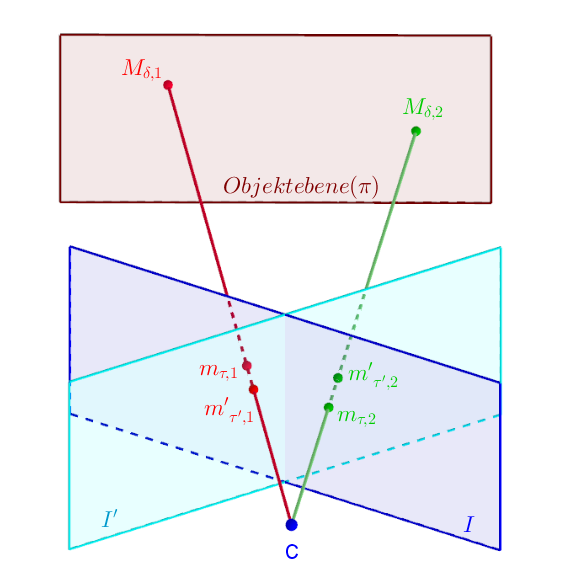
\includegraphics[width=\linewidth]{images/HomographyPZ_beschriftet.png}
	%	\caption{A really Awesome Image}
	\label{fig:HomographyPZFront}
	\endminipage\hfill
	\minipage{0.54\textwidth}
	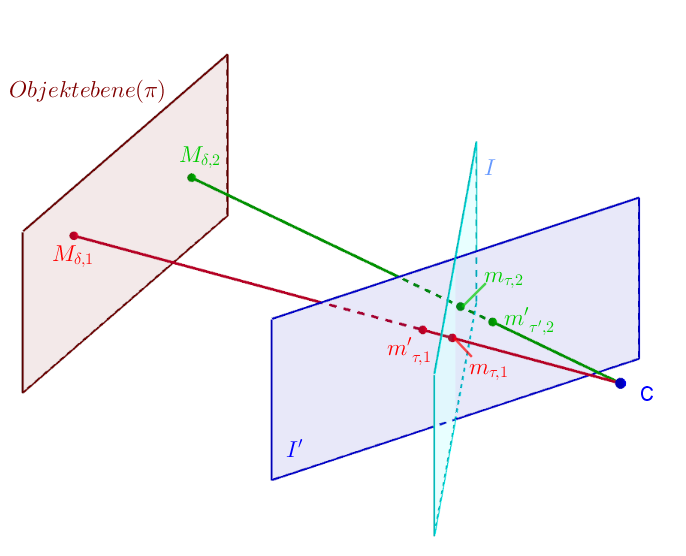
\includegraphics[width=\linewidth]{images/HomographyPZSide_beschriftet.png}
	%	\caption{A really Awesome Image}
	\label{fig:HomographyPZSide}
	\endminipage\hfill
	\caption{Die Abblildung zeigt zwei Aufnahmen einer um ihr Projektionszentrum $C$ gedrehten Kamera. Die zwei blauen Ebenen stellen jeweils die Bildebene vor und nach der Drehung dar sie wird einmal als Bildebene $(I,\tau)$ und einmal als Bildebene $(I',\tau')$ bezeichnet. Die Objektebene befindet sich im 3D-Raum, dementsprechend sind die Punkte $M_{1,\delta}$ und $M_{2,\delta}$ in homogenen 3D-Koordinaten gegeben. Die Punkte $m_{1,\tau}$ und $m_{2,\tau}$ sind die projizierten Puntke auf der Bildebene $(I,\tau)$ und Die Punkte $m_{1,\tau'}$ und $m_{2,\tau'}$ sind die projizierten Punkte auf der Bildebene $(I',\tau')$}
	\label{fig:homographyRotatedProjectionCenter}
\end{figure}

Um die Herleitung der Homographiematrix zu veranschaulichen, werden zwei unterschiedliche Fälle betrachtet. Der erste Fall ist in Abbildung \ref{fig:homographyRotatedProjectionCenter} gezeigt. Eine planare Szene im Raum soll auf die Bildebene $(I,\tau)$ einer Kamer projiziert werden, danach wird die Kamera um ihr Projektionszentrum gedreht die 3D-Objektpunkte somit auf die neu ausgerichtet Bildebene $(I,\tau')$ projiziert. Im zweiten Fall wird die Kamera nicht um ihr Projetionszentrum gedreht, sondern um einen definierten Drehpunkt, so dass zu der Rotation noch eine zusätzliche Translation der Kamera erfolgt. Für Fall eins wird zunächst angenommen, dass die Transformationsmatrizen $R$ und $R'$ sowie die Kameramatrizen $K$ und $K'$ bekannt sind. $m_\tau$ und $m'_{\tau'}$ sind die projizierten Punkte von $M_\delta$ auf den Bildebenen $(I,_tau)$ mit $\tau=(\hat{t_1},\hat{t_2},I)$ und $(I',_\tau')$ mit $\tau=(\hat{t_1}',\hat{t_2}',I)$. Die Kamerakoordiantensyteme werden definiert als $(C,\beta)$ mit $\beta = (\hat{b_1},\hat{b_2},\hat{b_3},C)$, wobei $\hat{b_3} = \overline{CI}$ ist und $(C',\beta')$ mit $\beta' = (\hat{b_1}',\hat{b_2}',\hat{b_3}',C')$, wobei $\hat{b_3}' = \overline{C'I'}$\cite{Elements}. 

% jedoch werden für die Rechnung eine andere Darstellung von $m$ und $m'$ verwendet. Die zu dem zweidimensionalen Bildebenkoordinatensystemen $(I,\tau)$ und $(I',\tau')$ korrespondierenden dreidimensionalen Kamerakoordinatensysteme $(C,\beta)$ mit $\beta = (\hat{b_1},\hat{b_2},\hat{b_3},\overline{IC})$ und $(C',\beta')$ mit $\beta' = (\hat{b_1}',\hat{b_2}',\hat{b_3}',\overline{I'C'})$ werden für die Herleitung verwendet.
% 
%  Diese Koordinatensysteme stellt die Bildebenenpunkte $m_\beta$ und $m'_{\beta'}$ wie im Kapitel \nameref{sec:basisTransformation} Gleichung 3.26 dar. Da in dieser Darstellung $\hat{b_1} = \hat{t_1} $ und $\hat{b_2} = \hat{t_2}$ ist, kommt es zu keinen Komplikationen. Die Koordinaten bleiben die selben nur werden sie aus dem 3D-Koordinatensystem der Kameras beschrieben und bekommen somit die Tiefenkomponeten $\zeta$ und $\zeta'$ wieder dazu. Der Grund warum diese Koordinatendarstellung für die Bildpunkte gewählt wird, ist das so vermieden wird, dass es zu konflikten der Dimensionen der Matrizen $R$ und $R'$ sowie $K$ und $K'$ und den Punkten $m_\beta$ und $m'_\beta$ kommt\cite{Elements}. 
  
Die folgenden Gleichungen 4.7 und 4.8 zeigen wieder die bereits bekannte Projektion eines 3D-Punktes auf die 2D-Bildebene, jedoch werden die projizierten Punkte $m_\beta$ und $m_{\beta'}$ noch bezüglich der dreidimensionalen Kamerakoordinatensysteme dargestellt. $\gamma$ und $\gamma'$ repräsentieren jeweils die Tiefe von $m_\beta$ und $m'_{\beta'}$, welche gegen Ende eliminiert wird\cite{Elements}.


\begin{gather}
\gamma \vec{m}_\beta = P \begin{bmatrix}\vec{M}_\delta\\1\end{bmatrix} = 
\begin{bmatrix}KR|-KR\vec{C}_\delta\end{bmatrix}\cdot \begin{bmatrix}\vec{M}\delta\\1\end{bmatrix} = KR(\vec{M}\delta - \vec{C}_\delta)\\
\gamma' \vec{m'_{\beta'}} = P' \begin{bmatrix}\vec{M'}_\delta\\1\end{bmatrix} = 
\begin{bmatrix}K'R'|-K'R'\vec{C}_\delta\end{bmatrix}\cdot \begin{bmatrix}\vec{M}\delta\\1\end{bmatrix} = K'R'(\vec{M}\delta - \vec{C}_\delta)
\end{gather}


Der Vektor $(\vec{M}\delta - \vec{C}_\delta)$, beschreibt die Verbindung zwischen dem Objektpunkt $M_\delta$  und dem Projektionszentrum $C_\delta$. Die Gleichungen 4.7 und 4.8 können auf Grund ihrer identischen Projektionszentren jeweils nach  $(\vec{M}\delta - \vec{C}_\delta)$ aufgelöst werden 

\begin{gather}
	\gamma RK^{-1}\vec{m_\beta} = \vec{M}_\delta - \vec{C}_\delta\\
	\gamma' R'K'^{-1}\vec{m'_{\beta'}} = \vec{M}_\delta - \vec{C}_\delta
\end{gather}

Da die Rechten seiten der Gleichungen 4.9 und 4.10 identisch sind, können die linken Seiten gleichgesetzt werden.

\begin{gather}
	\gamma' R'K'^{-1}\vec{m'_{\beta'}}=\gamma RK^{-1}\vec{m_\beta}\\
\end{gather}

Um nun die gewünschte Form von $m'_{\tau'} = Hm_{\tau}$ zu bekommen, wird die Gleichung nach $	\frac{\gamma'}{\gamma}\vec{m'_{\beta'}}$ aufgelöst.

\begin{gather}
	\frac{\gamma'}{\gamma}\vec{m'_{\beta'}} = K'R'R^TK^{-1}\vec{m}_\beta\\
\lambda \vec{m'}_{\beta'} = H\vec{m}_\beta\\
\leadsto m'_{\tau'} = H m_\tau
\end{gather}

Es Resultiert also dass wenn $\lambda = \frac{\gamma'}{\gamma}$, dann gilt dass $H = K'R'R^TK^{-1}$ gleicht. Gilt nun noch der Fall, dass $K = K'$ ist, dann reduziert sich $H$ zu $K^{-1}HK = R'R$, welches einer Rotation gleicht.\cite{Elements}. 




\section{Abbildungsunterschiede bei verschobenen Rotationsachsen}

Wie am Anfang des Kapitels erwähnt, sollen zwei verschiedene Fälle für die Homographie betrachtet werden. Der Grund sind, die unterschiedlichen Abbildungsmerkmale die bei einer Drehung um das Projektionszentrum und einer Drehung um einen definierten Drehpunkt entstehen. Die Frage ist, ob und wie sich beim zweiten Fall eine Homographiematrix herleiten lässt und in wie fern sie sich von der bereits bekannten Herleitung unterscheidet. Um zu veranschaulichen, was genau sich bei einer Drehung um ein Drehpunkt und der Drehung um das Projektionszentrum ändert, wurde eine Simulation geschrieben, welche die Abbildungsunterschiede beider Drehungen aufzeigt. Abbildung \ref{fig:SimulationAnfang} zeigt die Ausgangssituation der Simulation. In einen virtuellen Raum wurde eine Kamera platziert, welche auf ein Objekt gerichtet ist. Dieses Objekt besteht aus deinem Quadrat, das durch die schwarzen Eckpunkte begrenzt ist. In der Mitte des Quadrats wurde mit Rot der Mittelpunkt des Quadrats gekennzeichnet. Dieser Mittelpunkt symbolisiert den Drehpunkt um welchem sich die Kamera später drehen soll. 

\begin{minipage}{\linewidth}
	\centering
	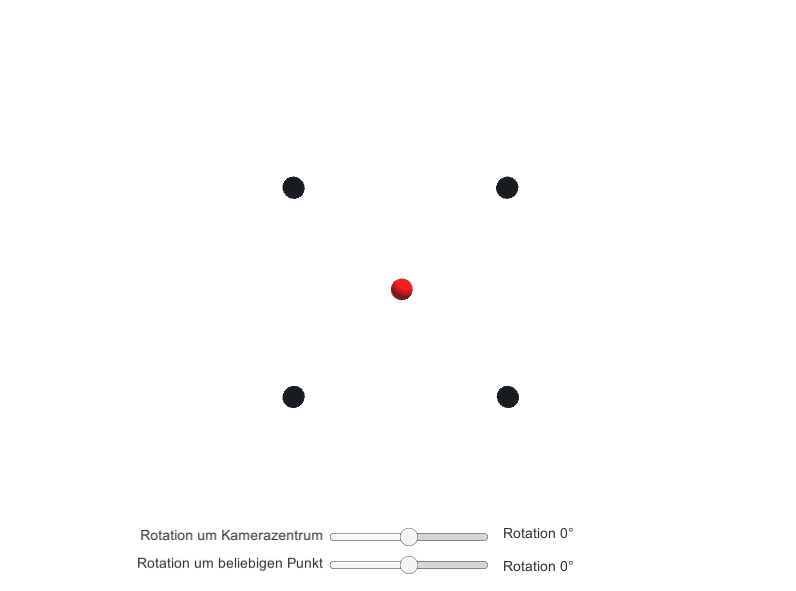
\includegraphics[width=.8\linewidth]{images/Ausgangslage.png}
	\captionof{figure}{Ausgangsituation der Simulation}
	\label{fig:SimulationAnfang}
\end{minipage}\\

%Im folgenden soll zunächst die Abbildungsunterschiede der entstehenden 2D-Bilder, bei den zwei genannten unterschiedlichen Fällen aufgezeigt werden.
%
%
%Bis jetzt wurden die Kameras jeweils nur um ihr Projektionszentrum gedreht, die Frage die jetzt noch im folgenden beantwortet werden soll ist, ob es ebenfalls möglich ist eine Homographiematrix für korrespondierende Punktepaare in einer Ebene aufzustellen, wenn eine Kamera um einen spezifischen Drehpunkt außerhalb der Kamera gedreht wurde. 
%
%In diesem Fall wären die beiden Projektionszentren $(C,\beta)$ und $(C',\beta')$ der Kameras nicht mehr identisch.  Des Weiteren soll geklärt werden, ob Punkte die bei der Drehung um das Projektionszentrum verdeckt bleiben auch bei einer Drehung um einen außerhalb der Kamera platzierten Drehpunkt verdeckt bleiben. In der Simulation ist der rote Punkte in der Mitte des Quadrats der Drehpunkt, wie in Abbildung \ref{fig:SimulationAnfang} dargestellt ist. 

Für die Simulation der unterschiedlichen Drehungen wurden zwei Schieberegler implementiert mit denen sich die Kamera einmal um ihr Projektionszentrum, und einmal um den Drehpunkt drehen lässt. Abbildung \ref{fig:DrehungProjektionszentrum} zeigt jeweils die entstehenden Bilder, wenn die Kamera um \ensuremath{20^\circ} beziehungsweise \ensuremath{-20^\circ} um das Projektionszentrum gedreht wurde.


\begin{minipage}{\linewidth}
	\centering
	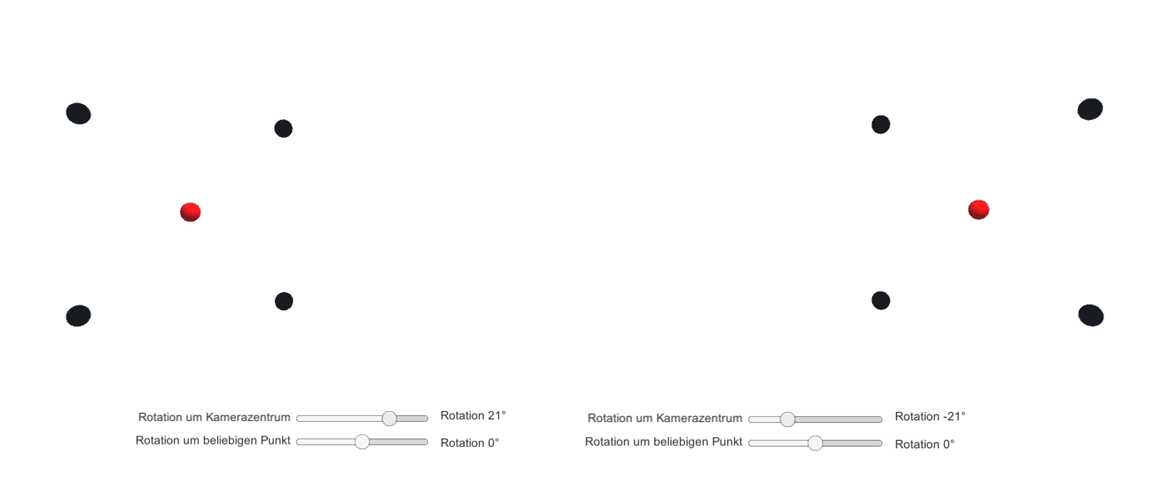
\includegraphics[width=1.\linewidth]{images/DrehungPZ.png}
	\captionof{figure}{Drehung um das Projektionszentrum}
	\label{fig:DrehungProjektionszentrum}
\end{minipage}\\ \\

Abbildung \ref{fig:DrehungDrehpunkt} zeigt die entstehenden Bilder, wenn die Kamera um \ensuremath{45^\circ} beziehungsweise \ensuremath{-45^\circ} um den Drehpunkt gedreht wurde. Wie sich zeigt ist hier ein weiterer grüner Punkt zu sehen welcher zu Testzwecken hinter dem roten Punkt platziert wurde sichtbar.

\begin{minipage}{\linewidth}
	\centering
	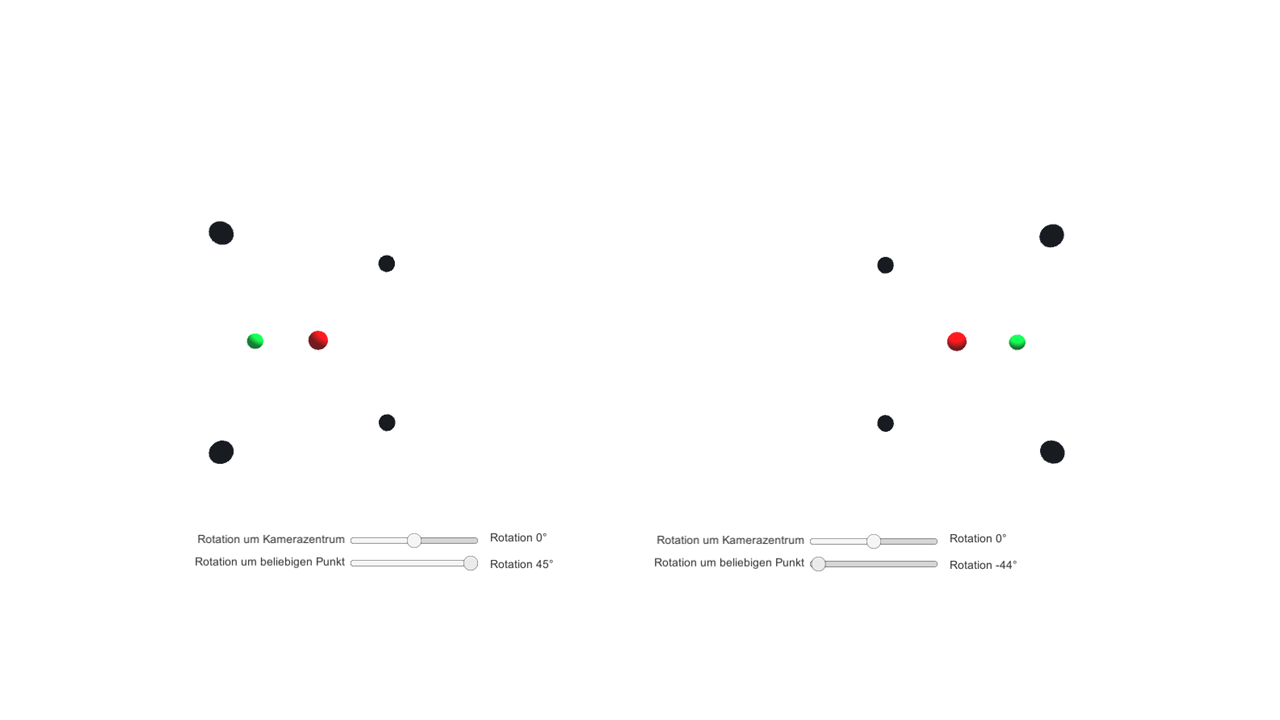
\includegraphics[width=1.\linewidth]{images/DrehungDZ.png}
	\captionof{figure}{Drehung um einen Drehpunkt. In diesem Beispiel wurde der rote Punkt als Drehpunkt verwendet}
	\label{fig:DrehungDrehpunkt}
\end{minipage}\\ 

Punkte die bei einer Drehung um das Projektionszentrum verdeckt bleiben, können bei einer Drehung um einen außerhalb der Kamera liegenden Drehpunkt sichtbar werden. Die Abbildungen \ref{fig:Strahlengang1} und \ref{fig:Strahlengang2} veranschaulichen anhand von Strahlenoptik, was der Grund für die Verdeckung ist. \\


\begin{figure}[!htb]
	\minipage{0.48\textwidth}
	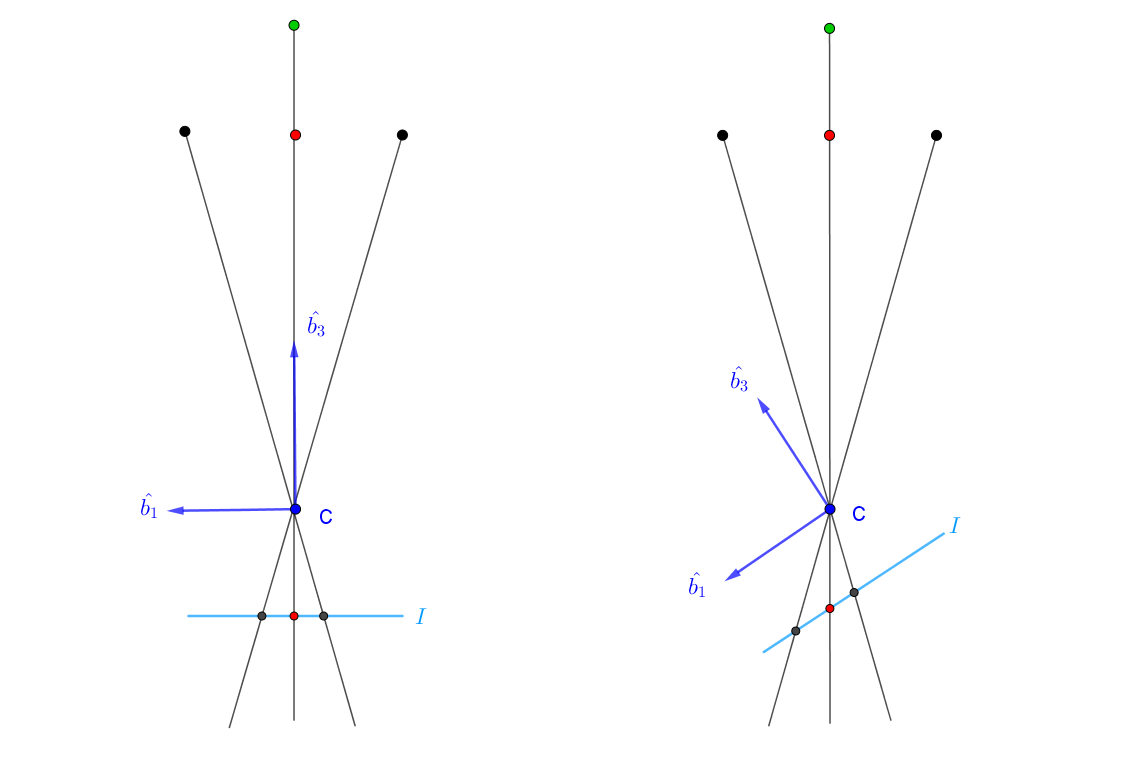
\includegraphics[width=\linewidth]{images/GrafikDrehungProjektionszentrum.png}
	\captionof{figure}{Strahlengang durch das Projektionszentrum. Auf der Abbildung ist erkennbar, dass der grüne Punkt auch nach der Drehung der Kamera um das Projektionszentrum vom roten Pukt verdeckt bleibt}
	\label{fig:Strahlengang1}
	\endminipage\hfill
	\minipage{0.5\textwidth}
	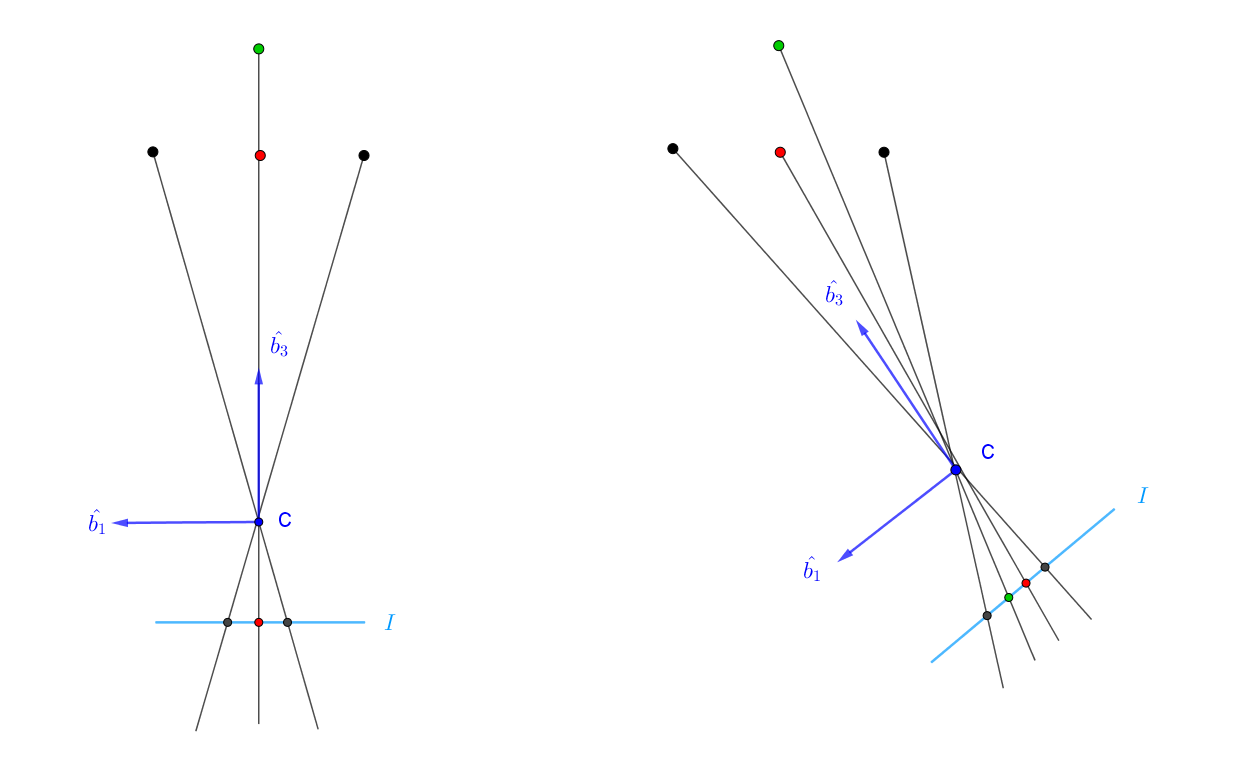
\includegraphics[width=\linewidth]{images/GrafikDrehungUmDrehpunkt.png}
		\captionof{figure}{Strahlengang durch das Projektionszentrum. Auf der Grafik ist erkennbar, dass der grüne Punkt nach der Drehung der Kamera um einen Drehpunkt, welcher in diesem Fall der rote Punkt darstellt, sichtbar wird.}
	\label{fig:Strahlengang2}
	\endminipage\hfill
\end{figure}

Die Bildebene ist in diesem Beispiel hinter dem Projektionszentrum platziert. Die Lage der Bildebene ist in sofern egal, dass es sei sie im gleichen Abstand vor oder hinter dem Projektionszentrum, immer zur selben Abbildung kommt. Jedoch ist die Abbildung, bei hinter dem Projektionszentrum platzierten Bildebene, auf dem Kopf abgebildet. Die Positionierung hinter das Projektionszentrum dient allein der Übersichtlichkeit der Abbildungen, im restlichen Verlauf der Arbeit wird die Bildebene immer vor das Projektionszentrum platziert um Verwirrungen zu vermeiden. Der grüne Punkt wurde nur als Beweis platziert, dass sich die entstehenden Abbildungen beider Fälle voneinander unterscheiden. Für den weiteren Verlauf wird er nicht weiter beachtet. Für die Homographie gelten nur die Punkte, welche sich im Raum auf einer Ebene befinden. Im folgenden wird eine Herleitung der Homographiematrix für den zweiten Fall aufgestellt. 

\begin{minipage}{\linewidth}
	\centering
	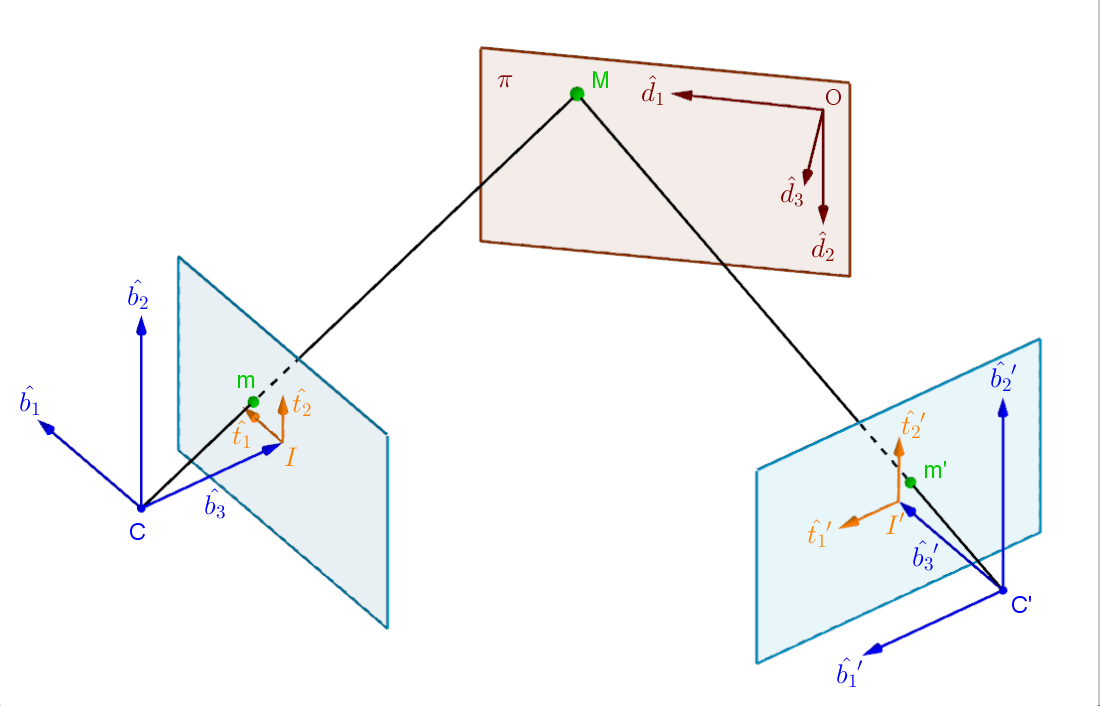
\includegraphics[width=0.8\linewidth]{images/HomographieDP_beschriftet.png}
	\captionof{figure}{Veranschaulichung der Homographie bei zwei verschieden translatierten und rotierten Kameras.}  
\end{minipage}\\

Angenommen es existiert eine Ebene $\pi$ im Raum mit einem Objektpunkt $M_\delta$ bezüglich eines Weltkoordinatensystems $(O,\delta)$ mit $\delta = (\hat{d_1},\hat{d_2},\hat{d_3},O)$. $\hat{d_1}$ und $\hat{d_2}$ spannen Die Ebene $\pi$ auf. Der Punkt $M_\delta$ wird nun mit den Projektionsmatrizen $P = [KR|-KR\vec{C}_\delta]$ und $P'=	[K'R'|-K'R'\vec{C}_\delta]$ in einen Punkt bezüglich der Bildebenen $(I,\tau)$ mit $\tau = (\hat{t_1}, \hat{t_2},I)$ und $(I',\tau')$ mit $\tau' = (\hat{t_1}', \hat{t_2}',I')$ projiziert. auch hier gilt wie im vorherigen Beispiel, dass die projizierten Bildkoordinaten als $m_\beta$ und $m'_{\beta'}$ der jeweiligen Kamerakoordinatensysteme $(C,\beta)$ mit $\beta = (\hat{b_1},\hat{b_2},\hat{b_3},C)$, wobei $\hat{b_3} = \overline{CI}$ und $(C',\beta')$ mit $\beta' = (\hat{b_1}',\hat{b_2}',\hat{b_3}',\overline{C'I'})$, wobei $\hat{b_3}' = \overline{C'O}$, dargestellt werden. Da der Ursprung des Weltkoordinatensystem $(O,\delta)$ auf der Ebene $\pi$ liegt und $\hat{d_1}$ und $\hat{d_2}$ diese aufspannen, gilt für den Punt $M_\delta$ auf $\pi$ $M_\delta = \begin{pmatrix}
x_{\hat{d_1}}\\
y_{\hat{d_2}}\\
0
\end{pmatrix}$. die Bezeichnungen $p_i$ und $p_i'$ stehen im folgenden für die einzelnen Spalten der Projektionsmatrizen $P$ und $P'$. Für die Projektion des Punktes $M_\delta$ in die Bildpunkte  $m_\beta$ und $m'_{\beta}$ bezüglich $(C,\beta)$ und $(C',\beta')$ gelten die folgenden beiden Gleichungen\cite{Elements}.


\begin{gather}
\gamma m_\beta = P \cdot 
\begin{bmatrix}
	M_\delta\\1
\end{bmatrix} = 
\begin{bmatrix}
	p_1&p_2&p_3&p_4
\end{bmatrix} \cdot
\begin{bmatrix}
	x_\delta\\y_\delta\\0\\1
\end{bmatrix}=
\begin{bmatrix}
	p_1&p_2&p_4
\end{bmatrix} \cdot
\begin{bmatrix}
	x_\delta\\y_\delta\\1
\end{bmatrix}=
G \vec{m}_\tau\\
\gamma' m'_{\beta'} = P \cdot 
\begin{bmatrix}
	M_\delta\\1
\end{bmatrix} = 
\begin{bmatrix}
	p'_1&p'_2&p'_3&p'_4
\end{bmatrix} \cdot
\begin{bmatrix}
	x_\delta\\y_\delta\\0\\1
\end{bmatrix}=
\begin{bmatrix}
	p'_1&p'_2&p'_4
\end{bmatrix} \cdot
\begin{bmatrix}
	x'_\delta\\y'_\delta\\1
\end{bmatrix}=
G' \vec{m}'_{\alpha}\\
\end{gather}\\

In diesem Prozess sind sowohl die zwei Matrizen $G$ und $G'$, sowie zwei weitere Koordinatensysteme $(C,\alpha)$ mit $\alpha = (\hat{d_1},\hat{d_2},\hat{d_4})$, wobei $\hat{d_4} = \overline{CO}$ und  $(C',\alpha')$ mit $\alpha' = (\hat{d_1},\hat{d_2},\hat{d_4}')$, wobei $\hat{d_4}' = \overline{C'O}$ entstanden\cite{Elements}.
Des Weiteren sind zwei neue Punkte $m_\alpha$ und $m'_{\alpha}$ entstanden, von denen behauptet wird, dass $\gamma m_\beta = G\cdot m_\alpha$ und $\gamma' m'_{\beta'} = G'\cdot m'_{\alpha'}$ gelte\cite{Elements}. Um dies zu testen werden $m_\alpha$ und $m'_{\alpha}$ anders formuliert.

\begin{gather}
	m_\alpha = M_\alpha + \overline{CO}_\alpha = M_{(\hat{d_1},\hat{d_2},\hat{d_4})} + \overline{CO}_{(\hat{d_1},\hat{d_2},\hat{d_4})} = \begin{pmatrix}
		x_\delta\\
		y_\delta\\
		1
	\end{pmatrix} \\
	m'_{\alpha'} = M_{\alpha'} + \overline{CO}_{\alpha'} = M_{(\hat{d_1},\hat{d_2},\hat{d_4}')} + \overline{CO}_{(\hat{d_1},\hat{d_2},\hat{d_4}')} = \begin{pmatrix}
	x_\delta\\
	y_\delta\\
	1
\end{pmatrix} 
\end{gather}

Aus Gleichungen 4.18 und 4.19 folgt dann, dass für alle Punkte in der Ebene $\pi$ gilt, dass $m_\alpha = m'_{\alpha}$. Woraus für die Punkte $\gamma m_\beta$ und $\gamma' m'_{\beta'}$ folgt, dass $\gamma m_\beta = G\cdot m_\alpha$ und $\gamma' m'_{\beta'} = G'\cdot m'_{\alpha'}$\cite{Elements}. Somit kann für $\gamma m_\beta$ und $\gamma' m'_{\beta'}$ folgende Beziehungsgleichung aufgestellt werden\cite{Elements}.

\begin{gather}
	\gamma' m'_{\beta'} = G' G^{-1} \gamma m_\beta
\end{gather}

Für $\frac{\gamma'}{\gamma} = \lambda$, kann Gleichung 4.20 dann wieder umformuliert werden in:

\begin{gather}
	\lambda m'_{\beta'} = H m_\beta\\
	\leadsto m'_{\tau'} = H m_\tau
\end{gather} 

Zwei projizierte Bilder einer Ebene sind also über eine Homographie $H$ miteinander verwandt, welche wiederum eine Kombination aus denjenigen Homographien ist, welche die jeweiligen Bilder mit der Ebene $\pi$ in Beziehung setzten\cite{Elements}.
 
\section{Berechnung der Homographiematrix aus Bildebenenkoordinaten}

Nachdem nun bekannt ist, wie eine Homographie Beziehungen zwischen projizierten Punkte beschreiben kann, wird im nächsten Schritt davon ausgegangen, dass die Transformationsmatrizen $R$ und $R'$ sowie die Kameramatrizen $K$ und $K'$ nicht bekannt sind. Es wird schematisch aufgezeigt, wie die Homographiematrix aus 2D-Bildpunkte gewonnen werden kann. Um eine Homographiematrix mit 
$H=
\begin{bmatrix}
h_{11}&h_{12}&h_{13}\\
h_{21}&h_{22}&h_{23}\\
h_{31}&h_{32}&h_{33}
\end{bmatrix}
$ zu erhalten werden die Punkte beider Kameras in eine Koeffizientenmatrix $A$ eingetragen, welche sich nach dem in den Gleichungen 4.25 bis 4.34 laufenden Schema aufstellen lässt. 

\begin{gather}
	H\cdot m_\tau = m'_{\tau}\\
	\begin{bmatrix}
		h_{11}&h_{12}&h_{13}\\
		h_{21}&h_{22}&h_{23}\\
		h_{31}&h_{32}&h_{33}
	\end{bmatrix}
	\cdot
	\begin{bmatrix}
		\\m_\tau\\\\
	\end{bmatrix}
	=
	\begin{bmatrix}
		\\m'_{\tau'}\\\\
	\end{bmatrix}\\
	\begin{bmatrix}
		h_{11}&h_{12}&h_{13}\\
		h_{21}&h_{22}&h_{23}\\
		h_{31}&h_{32}&h_{33}
	\end{bmatrix}
	\cdot
	\begin{bmatrix}
		x\\y\\z
	\end{bmatrix}
	=
	\begin{bmatrix}
		x'\\y'\\z'
	\end{bmatrix}
\end{gather}

Aus Gleichung 4.24 lässt sich ein Gleichungssystem mit zwölf Bekannten und neun unbekannten aufstellen.  

\begin{gather}
	h_{11}x+h_{12}y+h_{13}z= \lambda x'\\
	h_{21}x+h_{22}y+h_{23}z= \lambda y'\\
	h_{31}x+h_{32}y+h_{33}z= \lambda z'
\end{gather}

Da mit homogenen Koordinaten gearbeitet wird und somit $z$ und $z'$ = 1 sind, ergibt sich für die letzte Zeile $h_{31}x+h_{32}y+h_{33}z= 1$. Dieser Ausdruck kann in den ersten beiden Gleichungen für $\lambda$ eingesetzt werden. Pro Punktepaar $m_\tau$ und $m'_{\tau'}$ ergeben sich somit zwei Gleichungen. 

\begin{gather}
	h_{11}x+h_{12}y+h_{13}z= (h_{31}x+h_{32}y+h_{33}z) \cdot x'\\
	h_{21}x+h_{22}y+h_{23}z= (h_{31}x+h_{32}y+h_{33}z) \cdot y'
\end{gather}

Für den Aufbau von $A$ werden beide Ausdrücke noch nach Null aufgelöst, so dass sich die Gleichungen 4.34 und 4.35 aus 4.32 und 4.33 ergeben.

\begin{gather}
	h_{11}x+h_{12}y+h_{13}z -(h_{31}x+h_{32}y+h_{33}z) \cdot x'= 0 \\	h_{21}x+h_{22}y+h_{23}z-(h_{31}x+h_{32}y+h_{33}z) \cdot y'=0
\end{gather}
\begin{gather}
	\leadsto h_{11}x+h_{12}y+h_{13}z -h_{31}x\cdot x' - h_{32}y \cdot x'-h_{33}z\cdot x'= 0\\
	\leadsto h_{21}x+h_{22}y+h_{23}z-h_{31}x\cdot y -h_{32}y \cdot y -h_{33}z) \cdot y'=0
\end{gather}

Die enstandnen Gleichungen werden jetzt pro Punktepaar $m_\tau$ und $m'_{\tau'}$ in die Koeffizientmatrix $A$ nach folgendem Schema eingetragen.\cite{Elements,HZ,Schwarz,Heipke}

\begin{gather}
	\begin{pmatrix}
		x_1&y_1&1&0&0&0&x_1 x'_1&y_1 x'_1 & 1\cdot x'_1\\
		0&0&0&x_1&y_1&1&x_1 y'_1&y_1 y'_1 & 1\cdot y'_1\\
		&&&&&.&&&\\	
		&&&&&.&&&\\	
		&&&&&.&&&\\	
		x_i&y_i&1&0&0&0&x_i x'_i&y_i x'_i & 1\cdot x'_i\\
		0&0&0&x_i&y_i&1&x_i y'_i&y_i y'_i & 1\cdot y'_i
	\end{pmatrix}
	\cdot
	\begin{pmatrix}
		h1\\h2\\.\\.\\.\\hi
	\end{pmatrix}
	=0
\end{gather}

Wenn ein nicht überbestimmter Fall vorliegt, sprich wenn der Matrixrang von $A$ $\leq$ 8 beträgt, kann aus $A$ einfach der Kern bestimmt werden, um so die Einträge für die 3x3-Homographiematrix zu erhalten\cite{HZ,Elements,Schwarz}. Gesucht wird also ein Vektor $\vec{x}$, für den gilt das $H \cdot x = 0$. Der gesuchte Vektor $\vec{x}$ entspricht dem Kern der Koeffizientenmatrix und ist ein Spaltenvektor mit insgesamt neun Einträgen, welche in die 3x3-Homographiematrix eingetragen werden können\cite{HZ,Schwarz}. Tritt nun der Fall ein, dass es zu einem überbestimmtes System kommt, sprich wenn der Rang von $A$ größer 8 ist, so liefert die Bestimmung des Kerns kein eindeutiges Ergebnis mehr für den Vektor $\vec{x}$ und somit kann die Homographiematrix nicht eindeutig bestimmt werden\cite{HZ}. Für die Lösung überbestimmter Systeme wird die Singulärwertzerlegung angewandt\cite{HZ}\cite{Scholz}. Das bedeutet es wird nicht mehr derjenige Vektor $\vec{x}$ gesucht für den gilt $H \cdot x = 0$ ergibt, sondern es wird derjenige Vektor $\vec{x}$ gesucht, für den \ensuremath{\parallel H \cdot x\parallel} minimal wird\cite{HZ,Schwarz}. Die Singulärwertzerlegung von $A$ ist eine Faktorisierung der Matrix \ensuremath{A \in \mathbb{R}^{m \times n}} der Form \ensuremath{A = U \cdot S \cdot V^T} mit orthogonalen Matrizen \ensuremath{U \in \mathbb{R}^{m \times n}} und \ensuremath{V \in \mathbb{R}^{m \times n}} sowie mit einer Diagonalmatrix $S$. 

\begin{gather}
	S = \begin{pmatrix}
		s_1&&...&&0&0&&...&&0\\
		.&.&&&.&.&&&&.\\
		.&&.&&.&.&&&&.\\
		.&&&.&.&.&&&&.\\
		0&&...&&s_r&0&&...&&0\\	
		0&&...&&0&0&&...&&0\\
		.&&&&.&.&&&&.\\
		.&&&&.&.&&&&.\\	
		.&&&&.&.&&&&.\\	
		0&&...&&0&0&&...&&0\\	
	\end{pmatrix}
\end{gather}

Dabei soll für die diagonalen Singulärwerte in $S$ mit $s_1$ bis $s_r$ gelten, dass \ensuremath{s_1 \geq s_2 \geq ... \geq s_r \ge 0 }\cite{Scholz}. Nach dem Schema der Singulärwertszerlung, wird Matrix $A$ in die Form $USV^T$ zerlegt. Nach der Zerlegung sind die Diagonaleinträge von $S$ in einer absteigenden Reihenfolge sortiert. Die Spalte von $V^T$, welche mit dem kleinsten Singulärwert von $S$ korrespondiert, ergibt den Vektor $\vec{x}$, für den \ensuremath{\parallel H \cdot x\parallel} minimal wird. Somit gleichen die neun Einträge der Homographiematrix gleich der letzten Spalte von $V^T$. Beispielrechnungen, in denen die Homographiematrix einmal für den Fall des rotierten Projektionszentrums und einmal mit der Drehung um einen Drehpunkt mit durchgerechnet wurde befindet sich im  \nameref{sec:appendix} unter \ref{sec:AppendixHomographieRotationPZ} und \ref{sec:AppendixHomographieRotationDP}.




%\section{Punkte in unterschiedlichen Ebenen}
%
%The perspective
%projection of a point X by a camera with projection center C can be obtained
%geometrically in 3D affine space by taking all lines passing through the points C and
%X and finding the intersections with the (affine) image plane $\pi$.
%Three different situations may arise, Figure 9.1.\\
%
%1. If X 
%C, then there is an infinite number of lines passing through C 
%X,
%which intersect  $\pi$ in all its points, and therefore the projection of X contains
%the whole plane  $\pi$.\\
%
%2. If point Y != C lies in the plane  $\sigma$, which is parallel to  $\pi$ and passing through
%C, then the line passing trough C and Y (which there is exactly one) does not
%intersect the projection plane  $\pi$, and therefore, the projection of X is empty.\\
%
%3. If X does not lie in the plane  $\sigma$, then there is exactly one line passing through
%points C and X and this line intersects the projection plane  $\pi$ in exactly one
%point x. Hence the projection of X contains exactly one point x.\\
%
%Graphik zur Homographie anfertigen um einen Verlgeich der Punktebeziehungen zwischen epipolargeometrie und Homographie zu veranschaulichen 
%
%
%Überleitung zur Epipolargeometry.\\
%Warum kann hier keine Homographie benötigt werden\\
%was muss hier genutzt werden?\\
%
%$H$ berücksichtigt nicht die Tiefe der Punkte. Für $H$ müssen alle Punkte in einer Ebene liegen, nur so kann die Korrekte $H$ und somit die Translation und Rotation der Kamera berechnet werden. Werden Punkte aus einer 3D-Szene auf ein 2D Bild gemapped, sollte man denken, dass mit Hilfe von $H$ die Punkte auf diesen Bildern ineinander überführt werden könnten. Dem ist jedoch nicht so, da die Punkte in unterschiedlichen Tiefen liegen, werden sie natürlich anders auf eine 2D-Ebene gemapped als wenn sie sich in der selben Tiefen befinden würden. Was benötigt wird ist also die sogenannte Epipolargeometrie. Allem voran die Beziehungen von korrespondierenden Punkten zweier Bilder ausgedrückt durch die Fundamentalmatrix und der essentiellen Matrix.


 
%\section{Epipolargeometrie als Grundlage der Stereokalibrierung und Szenenrekonstrunktion}

%
%Die Epipolargeometrie beschreibt eine intrinsische projektive Geometrie zwischen zwei Bildern\cite{HZ}. Sie dient insbesondere zur Korrespondenzanalyse von Punkten aus Bildern und zur Gewinnung von 3-D-Informationen. Ohne Kenntnis der Kamerapositionen, kann mit Hilfe der Epipolargeometrie eine einfache Beziehung zwischen korrespondierenden Punkten hergestellt werden. Abbildung 3.12 zeigt, den Aufbau zweier Kameras mit ihren Projektionszentren $C$ und $C'$, deren Bildebenen $I$ und $I'$, welche vor den Projektionszentren platziert wurden. Die Bildebenen können sich auch hinter den Projektionszentren befinden, das hat letztendlich keinen Einfluss auf die geometrischen Beziehungen\cite{HZ}. Zu den Elementen der Epipolargeometrie gehören zum einen die Epipole $e$ und $e'$. Betrachtet man die Basislinie zwischen den beiden Projektionszentren, so entsteht der Epipol genau am Schnittpunkt der Verbindungslinie mit den jeweiligen Bildebenen. Tritt der Fall ein, dass die Basislinie parallel zu einer oder beiden Bildebenen ist, so kommt es zu keiner Abbildung des Epipols auf den entsprechenden Bildebenen, sondern der Epipol befindet sich in diesem Falle im unendlichen\cite{ZZGXr}. Das hat zur Folge, dass alle Epipolarlinien, welche durch den Epipol verlaufen, sich zueinander parallel anordnen. Epipolarlinien die Linien, welche durch einen Bildpunkt $m$ oder $m'$ und dem jeweiligen Epipol $e$ oder $e'$ des Bildes verlaufen. Der Korrespondierende Punkt zu $m$ ist $m'$ und die korrespondierende Epipolarlinie $l'$ zu $m$, ist diejenige Linie, welche durch $m'$ und $e'$ verläuft. 
%
%
%\begin{minipage}{\linewidth}
%	\centering
%	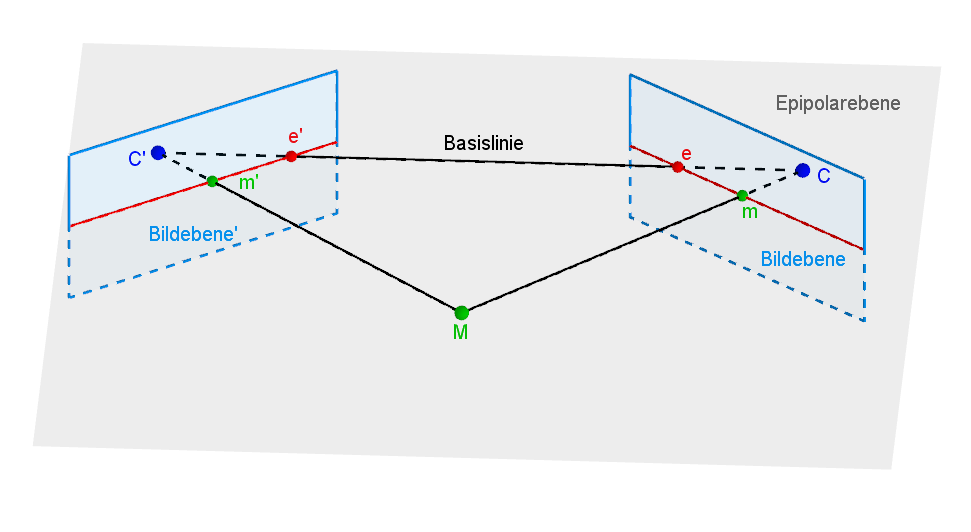
\includegraphics[width=1.\linewidth]{images/EpipolarGeoemtrieGrafik.png}
%	\captionof{figure}{Grafik zu den geometrischen Eigenschaften der Epipolargeometrie zwischen zweik Bildern. $C$ und $C'$ sind die Projektionszentren zweier Kameras. Beide Kameras besitzen jeweils eine Bildebene. Die Basislinien verbindet die Projektionszentren der Kameras. Der Punkt an welchem die Basislinie die Bildebenen schneidet, wird als Epipol bezeichnet. Durch den Epipol verlaufen alle Epipolarlinien des Bildes. $M$ ist der Objektpunkt im 3D-Raum und $m_1$ und $m_2$ sind die jeweiligen Abbildungen dieses Punktes auf den Bildebenen. Die Verbindungsvektoren zwischen $C, C'$ und $M$ bilden die sogenannte Epipolarebene\cite{Elements,HZ,ZZGXr}.}  
%\end{minipage}\\ \\
%
%
%Die Epipolarlinie $l'$, beinhaltet alle möglichen korrespondierenden Punkte zu $m$. Wenn $C$ auf seiner Bildebene $I$ einen Punkt $m$ abbildet, so erscheint dieser Punkt immer an der selben Stelle auf dem 2D - Bild, egal wie nah der Ursprüngliche 3D-Objektpunkt $M$ an $I$ befindet. Rein theoretisch, könnte der Originial Szenenpunkt $M$, sich überall auf der Verbindungslinie $\bar{Mm}$ befinden. Der Abgebildete Punkt $m$ wäre auf $I$ immer an der selben Stelle abgebildet. Fährt man nun mit $M$ die Verbindungslinie $\bar{Mm}$ entlang, dann ist $m$ immer an der selben Stelle auf $I$ zu sehen, während der korrespondierende Punkt $m'$ sich entlang der Epipolarlinie bewegen würde. Die Epipolargeometrie beschreibt also eine Beziehung zwischen einem Bildpunkt $m$ und dessen korrespondierender Epiplolarlinie $l'$, welche wiederum alle möglichen zu $m$ korrespondierenden Punkte $m'$ beinhaltet\cite{HZ,Zhang2014,ZZGXr}.\\
%
%
%
%\begin{minipage}{\linewidth}
%	\centering
%	\includegraphics[width=1.\linewidth]{images/EpipolarLinien.png}
%	\captionof{figure}{Die Objektpunkte $M_1, M_2$ und $M_3$ werden in $I'$ als $m'_1, m'_2$ und $m'_3$ abgebildet, während sie in $I$ immer den selben Bildpunkt $m_1$ ergeben.}  
%\end{minipage}\\ \\
%
%
%Die Epipolargeometrie lässt sich, ähnlich wie eines Homographiematrix, in einer 3x3-Matrix zusammenfassen. Diese ist jedoch singulär und besitzt somit nicht wie die Homographiematrix Rang 3 sondern Rang 2. Je nachdem ob ein ein kalibriertes oder unkalibriertes System vorliegen hat, handelt es sich entweder um die sogenannten Fundamental Matrix $F$ oder die Essentielle Matrix $E$ \cite{Elements,HZ,ZZPaper,Zhang2014,ZZGXr}. Von der Fundamentalmatrix $F$ ist dann die rede, wenn die intrinsischen Kameraparameter nicht bekannt sind, sprich wenn das System unkalibriert ist. In diesem Fall wird mit Bildpixelkoordinaten gearbeitet. Sind die intrinsischen Parameter bekannt, so wir $F$ zur essentiellen Matrix $E$ und es wird mit sogenannten normalisierten Bildkoordinaten gearbeitet\cite{ZZPaper}. Was genau die unterschiedlichen Koordinaten ausmacht, wird in Kapitel (KAPITELLINK) genauer erklärt. Mathematisch sagen die Matrizen $F$ und $E$ in Verbindung mit den korrespondierenden Punkten aus, ob für einen Bildpunkt $m$ in einer Kamera, dessen korrespondierender Bildpunkt $m'$ in der anderen Kamera auf der korrespondierenden Epipolarlinie liegt.  Das heißt, wenn $m'Fm = 0$ oder $\hat{m'}E\hat{m}= 0$, dann ist der sogenannte \textit{epipolar-constraint} erfüllt. Der \textit{epipolar-constraint} gibt somit Aufschluss darüber, ob $m'$ ein möglicher korrespondierender Punkt von $m$ ist. Dies ist nämlich genau dann der Fall, wenn $m'Fm = 0$ oder $\hat{m'}E\hat{m}= 0$ sind\cite{HZ,Zhang2014}. Ist der \textit{epipolar-constraint} erfüllt, so wird gleichzeitig der Suchaufwand nach weiteren Korrespondenzen reduziert, da somit nur noch eine eindimensionale Suche, entlang der Epipolarlinie, anstatt einer zweidimensionalen durchgeführt werden muss. Dieser neue \textit{contraint} wird auch als \textit{coplanarity constraint} oder Koplanaritätsbeschränkung bezeichnet. Dieser entsteht, da die Projektionszentren der Kameras und die korrespondierenden Bildpunkte auf ein und der selben Ebene liegen müssen \cite{Zhang2014}. Die Epipolargeometrie und die in ihr beinhalteten $constraints$, helfen bei der 3D-Szenenrekonstruktion. Szenenrekonstruktion ist dann möglich, wenn in einer Stereoaufnahme in beiden Bildern die zueinander gehörenden Bildpunkte lokalisiert wurden. Wird also eine Szene mit zwei Kameras aufgenommen, so liegen während der Aufnahme die aufgenommenen Objekpunkte, das Projektionszentrum und der zur Kamera gehörende Bildpunkt auf einer Linie. Wurde eine Objektpunkt nun zweimal aus verschiedenen Winkeln und/ oder Position aufgenommen, lassen sich nachdem die extrinsischen Parameter der Kameras ermittelt wurden, die Schnittpunkt der jeweiligen Linien aus Kamera eins und Kamera zwei berechnen. Diese Schnittpunkte ergeben den ursprünglichen Objektpunkt. Die Szene ist somit rekonstruiert\cite{Elements,ZZGXr,HZ}. 
%
%
%\section{Geometrische Erläuterung der Fundamentalmatrix und der Essentiellen Matrix }
%
%Nachdem die Theorie der geometrischen Hintergründe der Epipolargeometrie, bei der Stereokalibrierung und Szenerekonstruktion, erläutert wurden, wird nun der mathematische Hintergrund genauer aufgezeigt. Vor allem soll auf die Herleitung der neu eingeführten Fundamental Matrix $F$ und der essentiellen Matrix $E$ eingegangen werden. Diese spielen nämlich eine entscheidende Rolle bei der Rekonstruktion der Kamerapose und der Szenenrekonstruktion\cite{Elements, HZ}. $F$ und $E$ bilden jeweils eine singuläre 3x3-Matrix, welche die Geometrie zwischen den Bildpunkten $m_\tau$ und $m'_\tau$ auf $I$ und $I'$ und dem Objektpunkt $M_\delta$ im Raum beschreibt. Die Vektoren $\overline{CM} = (\vec{M}_\delta - \vec{C}_\delta),\, \overline{C'M} = (\vec{M}_\delta - \vec{C'}_\delta)$ und $\overline{CC'} = (\vec{C'}_\delta - \vec{C}_\delta)$ bilden das in Abbildung 3.12 sichtbare schwarze Dreieck. $F$ und $E$ fassen dieses Dreieck in ihren Matrizen zusammen. Um das ganze mathematisch zu erklären, wird ein Stereokameraufbau definiert. Ein Objektpunkt $M_\delta$ in Weltkoordinaten$(O,\delta)$ wird von zwei Kameras $C$ mit $(C,\beta)$ und $C'$ mit $(C',\beta')$ aufgenommen und auf deren Bildebenen $I$ und $I'$ als $m_\beta$ und $m'_\beta$ abgebildet. $C$ und $C'$ besitzen jeweils eine eigene Projektionsmatrix $P$ und $P'$. Anzumerken ist, dass die folgende Herleitung nach \cite{Elements} aufgestellt wurde.
%
%\begin{gather}
%	P = \begin{bmatrix}
%	KR|-KR\vec{C}_\delta
%	\end{bmatrix}\\
%	P' = \begin{bmatrix}
%	K'R'|-K'R'\vec{C'}_\delta
%	\end{bmatrix}
%\end{gather}
%
%$M$ wird mit $P$ und $P'$ auf die Bildebenen $I$ und $I'$ mit den jeweiligen Koordinatensystemen $I = (I,\tau)$ und $I'= (I',\tau')$ projiziert. Wichtig anzumerken, auch für den späteren Aufbau mit zwei Kameras unterschiedlicher Auflösung, ist, dass es sich bei den Koordinatensystemen von $I$ und $I'$ nicht um identische handeln muss.\cite{Elements} Es entstehen die Bildpunkte $\gamma m_\tau$ und $\gamma' m'_{\tau'}$ mit $\gamma \geq 0$ und $\gamma' \geq 0$. (gamma erklären)
%
%\begin{gather}
%	\gamma\vec{m}_\tau = P \begin{bmatrix}\vec{M}_\delta\\1\end{bmatrix}\\
%	\gamma\vec{m}_\tau = \begin{bmatrix}KR|-KR\vec{C}_\delta\end{bmatrix}\begin{bmatrix}\vec{M}_\delta\\1\end{bmatrix}\\
%	\gamma'\vec{m'}_{\tau'} = P' \begin{bmatrix}\vec{M}_\delta\\1\end{bmatrix}\\
%	\gamma'\vec{m'}_{\tau'} = \begin{bmatrix}K'R'|-K'R'\vec{C'}_\delta\end{bmatrix}\begin{bmatrix}\vec{M}_\delta\\1\end{bmatrix}\\
%\end{gather}
%
%$-KR\vec{C}_\delta$ und $-K'R'\vec{C'}_\delta$ verrechnet mit $M$ sind gleich den Vektorausdrücken $(\vec{M}_\delta - \vec{C}_\delta)$ und $(\vec{M}_\delta - \vec{C'}_\delta)$, welche die Verbindungslinie der beiden Projektionszentren mit dem Objektpunkt $M$ im Raum beschreiben.
%
%\begin{gather}
%	\gamma\vec{m}_\tau = KR(\vec{M}-\vec{C}_\delta)\\
%	\gamma'\vec{m'}_\tau = K'R'(\vec{M}-\vec{C'}_\delta)
%\end{gather}
%
%Gleichungen 3.89 und 3.90 werden nach $(\vec{M}-\vec{C}_\delta)$ und $(\vec{M}-\vec{C'}_\delta)$ aufgelöst.
%
%\begin{gather}
%	\gamma R^TK^{-1}\vec{m}_\tau = (\vec{M}-\vec{C}_\delta)\\
%	\gamma R'^TK'^{-1}\vec{m'}_{\tau'} = (\vec{M}-\vec{C'}_\delta)
%\end{gather}
%
%Wie bereits erwähnt ergibt sich aus den Vektoren $(\vec{M}_\delta - \vec{C}_\delta),\, (\vec{M}_\delta - \vec{C'}_\delta)$ und $(\vec{C'}_\delta - \vec{C}_\delta)$ das Dreieck aus Abbildung 3.12. Für das Dreieck kann, aus den drei Vektoren, die folgende Gleichung aufgestellt werden. 
%
%\begin{gather}
%	(\vec{C'}_\delta - \vec{C}_\delta) = (\vec{M}_\delta - \vec{C}_\delta) - (\vec{M}_\delta - \vec{C'}_\delta)
%\end{gather}
%
%$(\vec{M}-\vec{C}_\delta)$ und $(\vec{M} - \vec{C'}_\delta)$ können durch die Ausdrücke in den Gleichungen 3.91 und 3.92 ersetzt werden.
%
%\begin{gather}
%		(\vec{C'}_\delta - \vec{C}_\delta) = \gamma R^TK^{-1}\vec{m}_\tau - \gamma R'^TK'^{-1}\vec{m'}_{\tau'}
%\end{gather}
%
%Es gilt $\gamma \geq 0$ und $\gamma' \geq 0$, sie stehen für die Teife von $m$ und $m'$ und können mit Hilfe des Kreuzproduktes eliminiert werden\cite{Elements}. Zunächst wird $(\vec{C}'_\delta - \vec{C}_\delta)$ auf die rechte Seite gebracht, so dass die Gleichung nach Null aufgelöst wird.
%
%
%\begin{gather}
%	\begin{bmatrix}\vec{C'}_\delta - \vec{C}_\delta\end{bmatrix}_\times \gamma R^TK^{-1}\vec{m}_\tau - 
%	\begin{bmatrix}	\vec{C'}_\delta - \vec{C}_\delta\end{bmatrix}_\times \gamma' R'^TK'^{-1} \vec{m'}_{\tau'} =  0
%\end{gather}
%
%Gleichung 3.95 wird von links mit $\gamma' \vec{x'}^T_{\tau'}K'^{-T}R'$. Somit kann eine der beiden Schiefsymmetrischen Matrizen aus der Gleichung eliminiert werden. 
%
%\begin{gather}
%	\gamma' \vec{m'}_{\tau'} K'^{-T}R' \begin{bmatrix}	\vec{C'}_\delta - \vec{C}_\delta\end{bmatrix}_\times \gamma R^TK^{-1}\vec{m}_\tau = 0
%\end{gather}
%
%Da $\gamma \geq 0$ und $\gamma' \geq 0$, kann für Gleichung 3.96 auch folgendes geschrieben werden.
%
%\begin{gather}
%	 \vec{m'}_{\tau'} K'^{-T}R' \begin{bmatrix}	\vec{C'}_\delta - \vec{C}_\delta\end{bmatrix}_\times R^TK^{-1}\vec{m}_\tau = 0
%\end{gather}
%
%Aus Gleichung 3.97 können nun die Matrizen $F$ und $E$ ausgelesen werden. Bei $E$ handelt es sich um einen Kalibrierten Fall, dass bedeutet dass sowohl $K$ als auch $K'$ bekannt sind und die normalisierten Bildkoordinaten $\vec{\hat{m}}$ und $\vec{\hat{m}}'$  durch multiplikation mit $K$ und $K'$ entstehen. $E$ selbst fässt die Schiefsymmetrische Matrix $[\vec{C'}_\delta - \vec{C}_\delta]_\times$ und die beiden Transformationsmatrizen $R$ und $R'$ zusammen. 
%
%\begin{gather}
%	\vec{m'}_{\tau'}^T K'^{-T}EK^{-1}\vec{m}_\tau = 0\\
%	\vec{\hat{m}}_\tau^T E \vec{\hat{m}}'_{\tau'} = 0
%\end{gather}
%
%Matrix $E$ wird zu $F$, wenn es sich um einen unkalibrierten Fall handelt. Unkalibriert bedeutet, dass $K$ und $K'$ nicht bekannt sind, die Informationen zu $K$ und $K'$ in $F$ befinden. Werden $K$ und $K'$ zu $E'$ multipliziert, wird $E$ zu $F$. 
%
%\begin{gather}
%	\vec{m'}_{\tau'}^T K'^{-T}EK^{-1}\vec{m}_\tau = 0\\
%		\vec{m'}_{\tau'}^T F\vec{m}_\tau = 0
%\end{gather}
%
%$F$ und $E$, fassen die komplette Epipoloargeometrie, sprich externe und interne Parameter, sowie die geometrische Beziehung der jeweiligen Bildpunkte zu den 3-D Objektpunkten in einer 3x3-Matrix zusammen. Für $F$ und $E$ gibt es nicht nur eine Lösung. Werden $F$ oder $E$ Beispielsweise über den \textit{eight-Point-Algorithm} ermittelt, so sind die entstehenden 3x3-Matrixen und jedes vielfache von diesen gültige Lösungen für $F$ und $E$\cite{HZ,HZ8}. \textcolor{red}{Noch herausfinden ob das mit den Tiefen $\gamma$ und $\gamma'$ zusammenhängt!!}. Mit $F$ und $E$ kann wie bereits nachgeprüft werden, ob der \textit{epipolar-constraint} $m'^TFm = o$ oder $\hat{m'}^TE\hat{m} = 0$ zwischen zwei Bildpunkte gilt. Des weiteren können Epipole $e$ und $e'$ und Epipolarlinien $l$ und $l'$ ausfindig gemacht werden, sobald $E$ oder $F$ bekannt ist\cite{HZ,Elements,HZ8,ZZGXr}. Um die zu $m$ oder $m'$ korrespondierende Epipolarlinie $l'$ oder $l$ zu berechnen gilt:
%
%\begin{gather}
%l' = Fm\\
%l = F^Tm'
%\end{gather} 
%
%Um die Epipole $e$ und $e'$ zu berechnen die Gleichungen 3.103 und 3.104 erfüllt sein. Für $e$ reicht es also den rechten Nullraum von F zu bestimmen und für $e'$ muss dementsprechend der linke Nullraum von $F$ gefunden werden. 
%
%\begin{gather}
%	Fe = 0\\
%	F^Te' = 0
%\end{gather}
%
%Die Matrizen $F$ und $E$ sind die ausschlaggebenden Elemente, wenn es um die rekonstruktion der Kameraorientierungen und der Rekonstruktion der Szene geht. In beiden folgenden Kapitel werden zwei Beispiele zur Findung der exterenen Kameraparameter und der Szenenrekonstruktion aufgezeigt. Beim ersten Beispiel handelt es sich um ein Minimalbeispiel mit synthetisch erzeugten reinen Daten, um die theoretische Funktionalität des Algorithmus zu beweisen. Im zweiten Beispiel, wird der Algorithmus, mit einigen Anpassungen an die Realverhältnisse, auf Stereobildpaare, aufgenommen von zwei verschiedenen Kameras, angewandt. Die implementierten Algotithmen ermitteln aus einem Satz korrespondierender Bildpunkte die Fundamental Matrix und die essentielle Matrix mit Hilfe des sogenannten \textit{8-Point-Alhorithm}, Im Anschluss werden dann die externen Kameraparameter ermittelt und die Szene mit einem Triangulationsverfahren rekonstruiert. 
%
